%% Modelování a simulace
%% Týmový projekt - Půjčovna vodáckého vybavení
%% Technická zpráva
%% autor: Tomáš Barták
%% date: 21. 04. 2024

\documentclass[a4paper, 12pt, hidelinks]{article}
\usepackage[left=2cm, top=3cm, text={17cm, 24cm}]{geometry}
\usepackage[czech]{babel}
\usepackage[utf8]{inputenc}
\usepackage[T1]{fontenc}
\usepackage{times}
\usepackage{listings}
\usepackage{xcolor}
\usepackage{graphicx}
\usepackage{fancyhdr}
\usepackage{url}
\usepackage[linesnumbered, ruled, czech, noline, longend]{algorithm2e}
\usepackage{amsmath}

\pagestyle{fancy}
\setlength{\headheight}{14.49998pt}

\begin{document}

\begin{titlepage}
	\begin{center}
		\textsc{
			\Huge{Vysoké učení technické v~Brně}\\
			\huge{Fakulta informačních technologií\\}
		}
		\vspace{\stretch{0.382}}
		\LARGE{
			Technická zpráva\\
			\Huge{T6 - Půjčovna vodáckého vybavení}\\
		}
		\vspace{\stretch{0.618}}
	\end{center}
	{\Large{
		\hfill
		Tomáš Barták (xbarta51)

        \today
        \hfill
        Norman Babiak (xbabia01)

		}
	}
\end{titlepage}

\rhead{}
\newpage
\tableofcontents
\newpage
\section{Úvod}
Tato práce se zabývá implementací modelu [1, snímek 7] půjčovny vodáckého vybavení, sídlící v Brně, na ulici Labská 2106, pod názvem SportRonTour, a následným zkoumáním chování namodelovaného systému [1, snímek 7]. Půjčovna je k dispozici dle potřeb klientů, ale tato simulace [1, snímek 8] bude zaměřená především na aktivní sezónu, která dle získaných dat trvá zhruba od půlky dubna, do konce října. 

Model půjčovny vodáckého vybavení je založen na základě zjištěných dat a je cíleno na co nejrealističtější přísun zákazníků, a to včetně skupin s vysokým odběrem dostupného vybavení (zájezdů). Na základě experimentů [1, snímek 276] lze určit ideální počet dostupného vybavení, zda-li je systém schopen zvládnout nárazový příchod většího množství zákazníků ovlivněný reklamní kampaní a podobně.

\subsection{Autoři a zdroje}
Autory průzkumu, následného návrhu a implementace modelu jsou Tomáš Barták a Norman Babiak. Přesto, že neexistuje příliš velké množství odborných zdrojů literatury pro tohle téma, tak informace a statistiky jsou založené na reálných datech a faktech, jak z osobní zkušenosti při občasné výpomoci ve vodácké půjčovně, tak zároveň všechna data a procesy byly konzultovány a doplněny dle rad a informací dlouholetého majitele půjčovny SportRonTour, Ronalda Bartáka. 

\subsection{Ověření validity modelu}
Validita modelu [1, snímek 37] byla ověřená pomocí základních experimentů, kde výsledky byly porovnávány se zpětnou vazbou od firmy, která nám poskytovala konzultace a informace o fungování. 

\newpage

\section{Rozbor tématu, použitých metod a technologií}
Informace a data k tématu byly získány jak z osobních poznatků, tak z konzultace s majitelem půjčovny vodáckého vybavení.

Zákazníci během aktivní sezóny, která trvá cca od půlky dubna do konce října přicházejí do budovy půjčovny, která má otevřeno v závislosti na předchozí domluvě se zákazníkem (je potřeba dopředu vytvořit rezervaci). Lodě si půjčují jak jednotlivci (cca po 2 kusech), tak i větší skupinky (školy, zájezdy, ...), které chodí sice asi 20x méně než jednotlivci, ale mají velký odběr lodí na jednu rezervaci (cca 20 lodí). V případě, že se stane, že by dva různí zákazníci chtěli vypůjčit vybavení ve stejnou dobu, pak jeden z nich bude muset počkat a zařadit se do fronty, do doby než bude obsluha opět k dispozici, aby bylo možné vybavení půjčit. Samotná obsluha zahrnuje nafouknutí zarezervovaných lodí, předvedením, vyfouknutím, sbalením, podpis smlouvy a mnoho dalších.

Při návratu vybavení je nutno lodě zkontrolovat (nafouknutí, vyfouknutí, sbalení), přičemž průměrně u jednoho z dvaceti kusů vybavení se vyskytne nějaké nadstandardní opotřebení, či jiné poškození, které je nutno poslat k opravě a náležitě se zákazníkem urovnat škodu. 

\subsection{Použité metody a technologie}
Systém hromadné obsluhy [1, snímek 139] půjčovny s vodáckým vybavením je popsán grafovým popisem [4, strana 31] formou Petriho sítě [1, snímek 122], kterou tvoří graf popisující stavy a přechody mezi nimi, jsou ideální, protože umožňují vyjádření paralelismu a nedeterminismu.

Jako implementační jazyk modelu byl zvolen programovací jazyk C++, se simulační knihovnou SIMLIB[2], která obsahuje předem nadefinované funkce pro práce s procesy [1, snímek 124] a frontami [1, snímek 141].

Pro sestavení a překlad projektu je využíván nástroj GNUMake a soubor Makefile, jako kompilátor jsme zvolili g++.

\subsection{Původ použitých technologií}
Jak již zaznělo v předchozím textu, pro simulování jsme využili knihovny SIMLIB (pod licencí GNU LGPL), jejichž autory jsou Petr Peringer, David Leska a David Martinek [2]. Pro verzování projektu byl použitý git. Projekt byl uložen na platformě Github [3].

\newpage

\section{Koncepce}
Tato kapitola se zabývá popisem návrhu konceptuálního modelu [1, snímek 48] systému.

Pro potřeby modelu jsme zanedbali fakt, že obsluha není stabilně v půjčovně, ale vynecháním této informace se model nijak nezmění, protože obsluha na základě předchozí rezervace se zákazníkem je vždy s předstihem v budově půjčovny, takže čekání zákazníka to nijak neovlivní.

Dalším zjednodušením je zanedbání rezervace ostatního vybavení mimo lodě, jelikož půjčovna má naddimenzované množství ostatního vybavení a také má dva typy lodí místo jednoho (obě se stejnou kapacitou), což znamená, že i kdybychom počítali na každou loď 3 kusy vybavení (což je maximální kapacita lodi), pak by pořád v půjčovně vybavení zbylo po půjčení všech lodí. Vybavení v půjčovně musí být tolik, aby bylo možné vybírat z jednotlivých velikostí.

Posledním zjednodušením je variabilita aktivní sezóny, v reálu se může začátek a konec sezóny lišit o 1-2 týdny, ale model to významně neovlivní. Při větším množství sezón se tato doba ustálí na použité době od půlky dubna do konce října, tedy 6,5 měsíce (měsíc považujeme jako 30 dní).

Tvorba samotného modelu je založena na informacích o procesech a datech získaných od našeho odborného konzultanta, v podobě majitele vodácké půjčovny.

\subsection{Konceptuální model}
Pro jednoduchost a přehlednost jsme se rozhodli konceptuální model rozdělit na bloky, které budou v následujícím textu popsány podrobněji.

Abstraktní model znázorňuje tok rezervací a vybavení v probíhající sezóně. Po vytvoření rezervace si zákazník půjčí předem domluvené množství lodí. Po uplynutí časového intervalu pro půjčení lodě přinese zpátky a zkontroluje se jestli jsou poškozené. V případě že ano, lodě jsou vysušené a poslané do opravny, jinak se jenom vysuší. Po dokončení těchto procesů se lodě vrátí do skladu.

\begin{figure}[h]
    \centering
    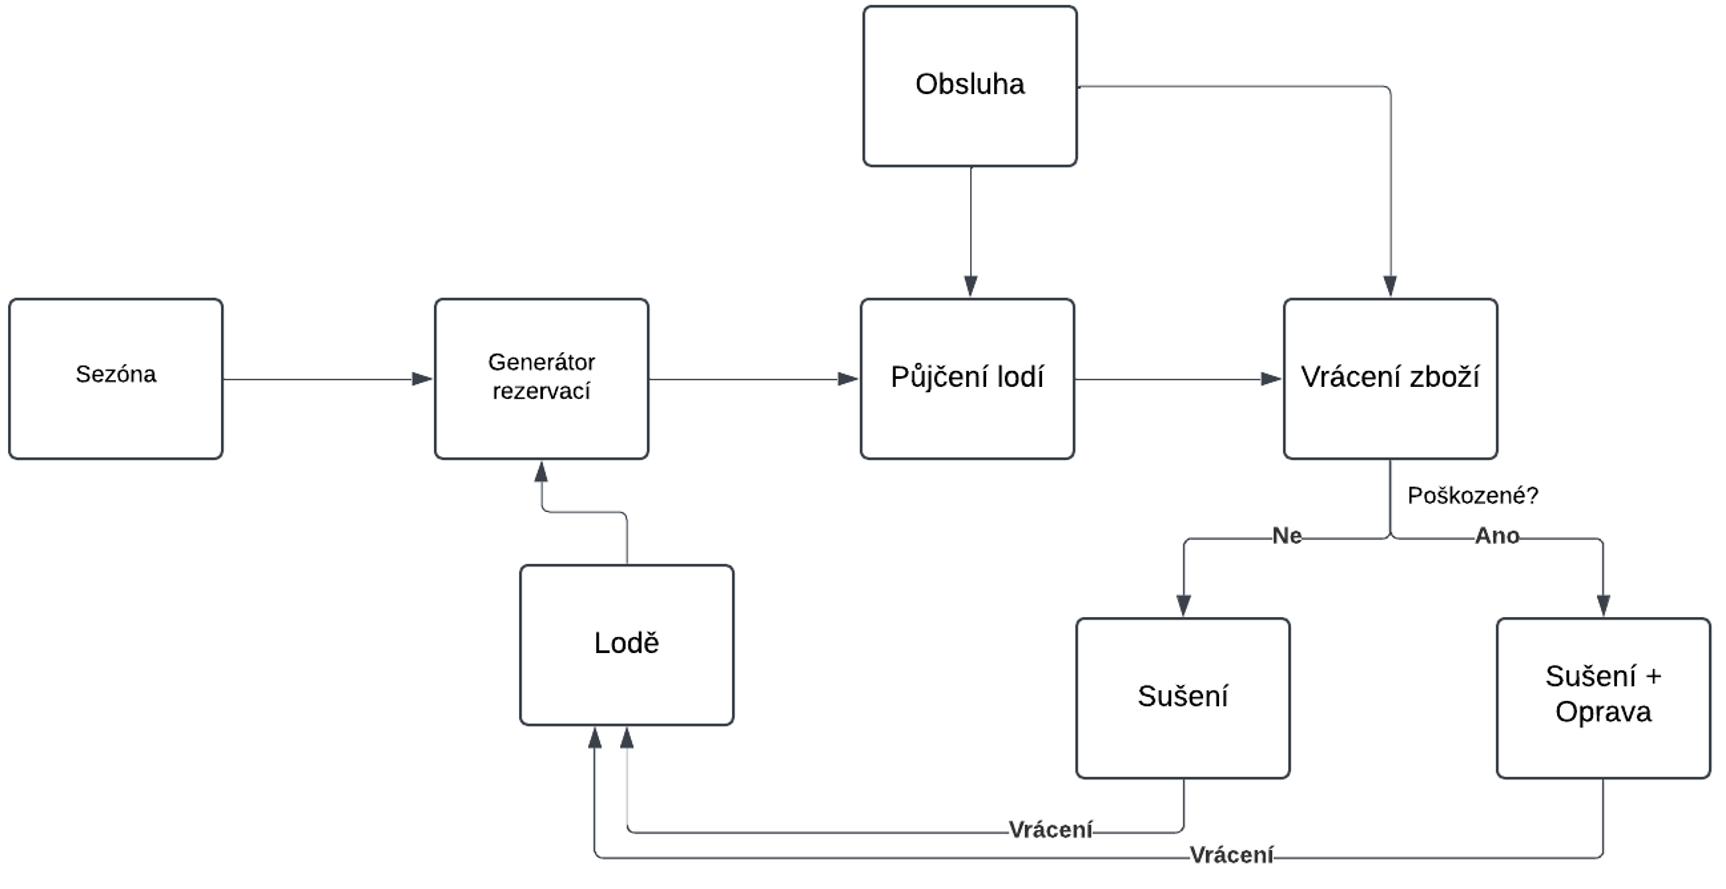
\includegraphics[width=1.0\linewidth]{images/abstrakt.png}
    \caption{Abstraktní model systému}
    \label{fig:abstract}
\end{figure}

\subsubsection{Sezónní dostupnost}

Následující blok Petriho sítě popisuje způsob vypínání generátorů pro rezervace (ukončení příchodu nových zákazníků), který je řízen sezónním cyklem. Aktivní sezóna trvá 6 a půl měsíce (od půlky dubna do konce října). Po uplynutí této doby již nevznikají nové rezervace, generátory jsou vypnuty, a to až do okamžiku začátku nové sezóny, která začne po dalších 5 a půl měsících. Tento sezónní cyklus se každý rok opakuje.

\begin{figure}[h]
    \centering
    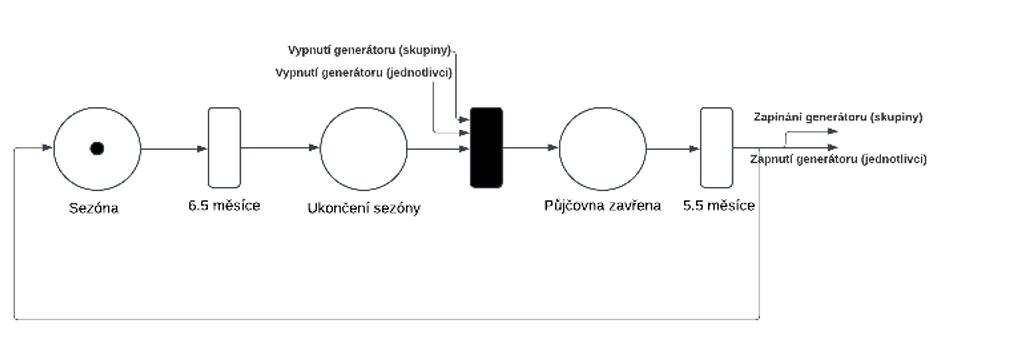
\includegraphics[width=0.85\linewidth]{images/sezona.png}
    \caption{Sezóna pro vypínání a zapínání generátorů}
    \label{fig:season}
\end{figure}

\subsubsection{Generátor zákazníků/rezervací}

Tento blok znázorňuje vznik rezervací a navazuje na předchozí blok \ref{fig:season}, který slouží pro vypnutí a zapnutí generátoru podle současné sezóny. Zároveň se při vytváření rezervace musí zkontrolovat stav dostupnosti vybavení, aby nebylo možné zákazníkům přislíbit a zarezervovat počet vybavení, který pro ně není dostupný. Jakmile je vybavení dostupné, tak je potřeba vymyslet termín, kdy si zákazník chce vybavení půjčit. Po nastání této doby zákazník přichází do půjčovny a pokud je nějaký zákazník již obsluhován, tak se zařadí do fronty, kde čeká, než ho obsluha bude moci přijmout.

\begin{figure}[h]
    \centering
    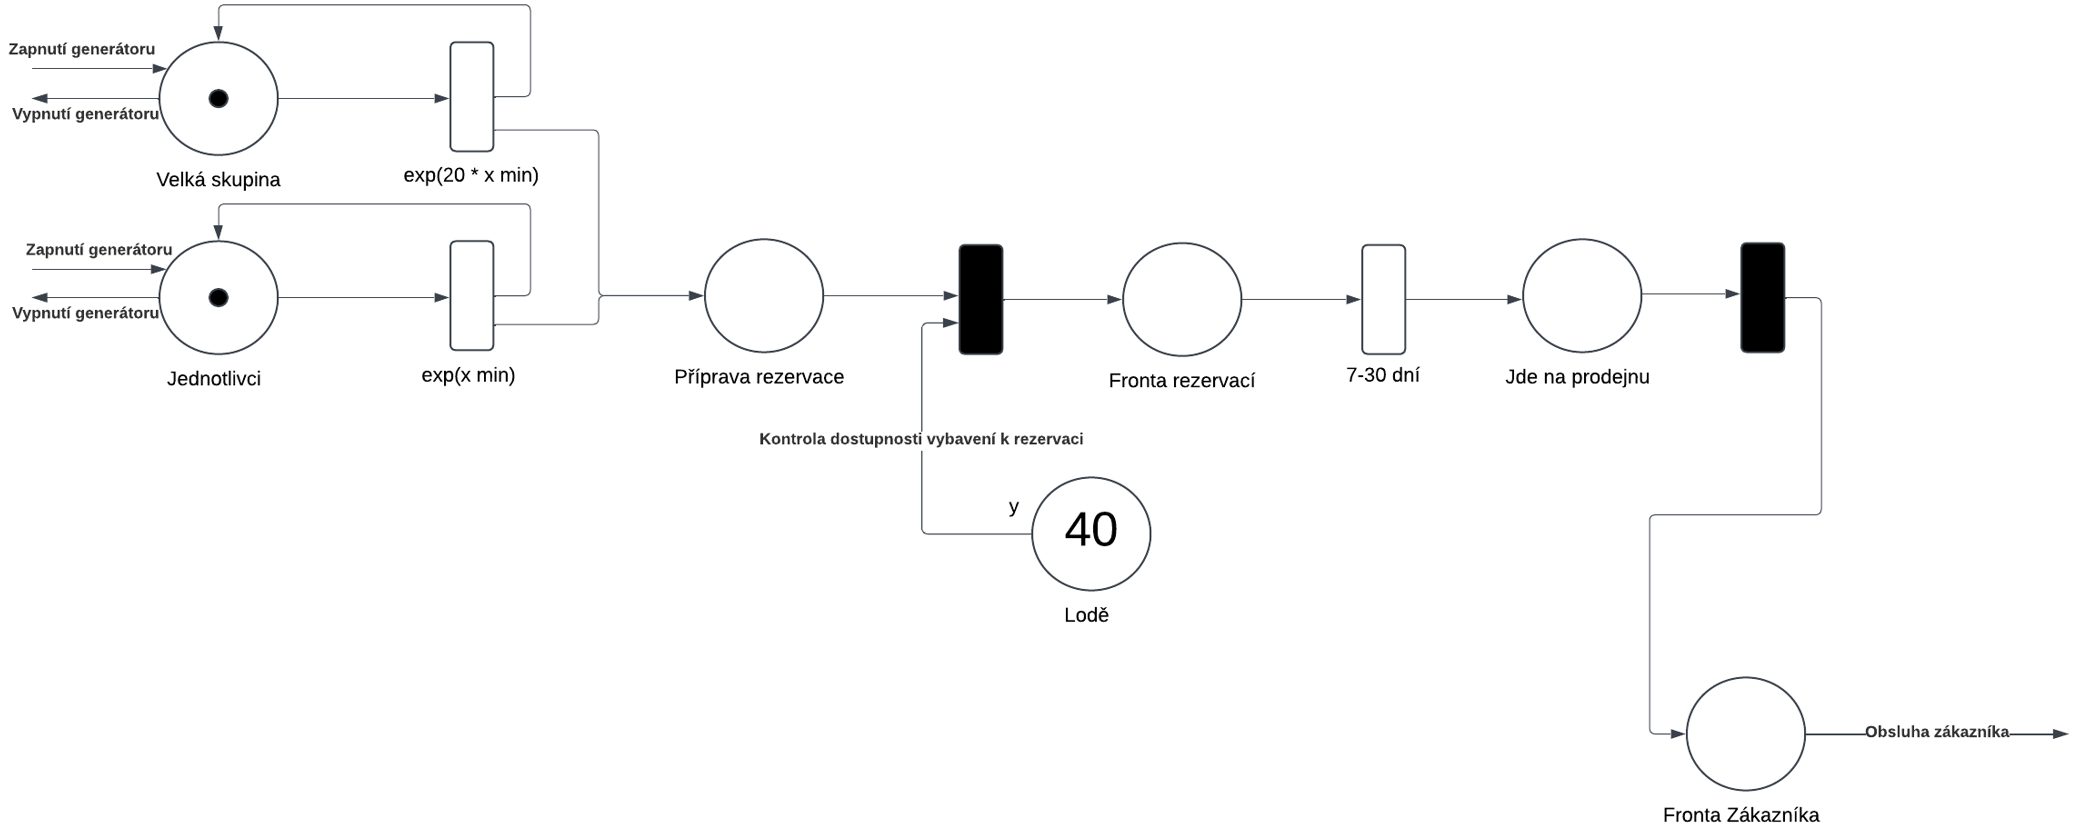
\includegraphics[width=1.0\linewidth]{images/rezervace.png}
    \caption{Generátor zákazníků (rezervací)}
    \label{fig:reservation}
\end{figure}

\newpage

\subsubsection{Obsluha zákazníka}

Blok znázorněný Petriho sítí na obrázku \ref{fig:service} slouží k popisu průběhu samotné obsluhy při vypůjčování vybavení. Zaměstnanec obsluhuje postupně zákazníky z fronty (FIFO [1, snímek 141]), kde je potřeba nafouknout všechny lodě, provést poučení o vypůjčeném vybavení, předvést, že lodě nemají žádné známky nadměrného opotřebení, případně nějaké další škody. Následně se lodě musí opět vyfouknout, sbalit a vyřídit právní dokumenty (sepsat smlouvu, zaplatit doplatek, ...). Poté se obsluha může jít věnovat dalším zákazníkům z fronty. Zákazník si vybavení půjčí na zvolenou dobu a po uplynutí této doby je nutné ho zase vrátit zpět do půjčovny.

\begin{figure}[h]
    \centering
    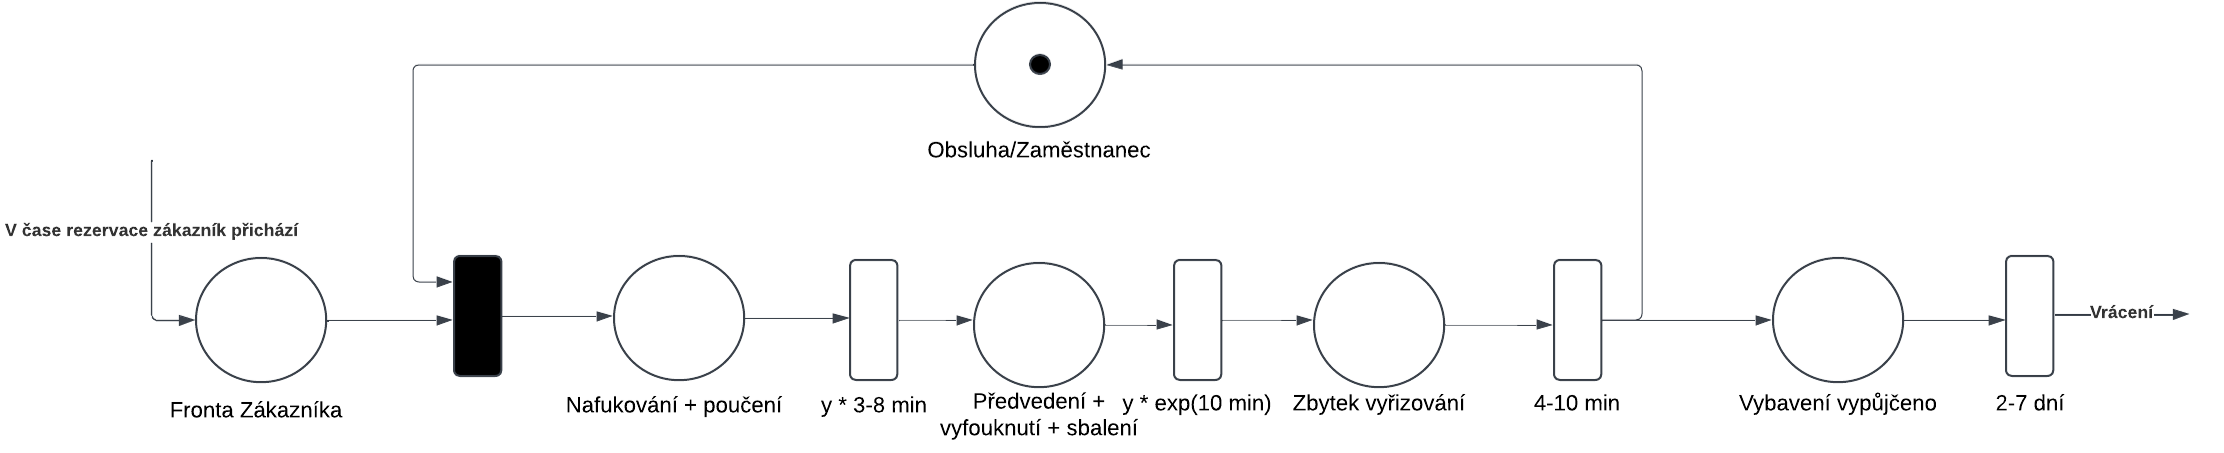
\includegraphics[width=1.0\linewidth]{images/obsluha.png}
    \caption{Obsluha zákazníka}
    \label{fig:service}
\end{figure}

\subsubsection{Vrácení zboží}

Blok znázorňující popis, co se děje po uplynutí doby vypůjčení vybavení je zobrazený na obrázku \ref{fig:return}. Na začátku je potřeba, aby všechno vybavení bylo opět zkontrolováno obsluhou, zda-li je vše v pořádku, jestli došlo k nadměrnému opotřebení, ztrátě či dalším jevům, které vyžadují opravu vybavení nebo jejich kompletní výměnu. K nutnosti vybavení vyměnit z důvodu nadměrného opotřebení a podobných jevů dojde v průměru u jednoho z 20 vypůjčených vybavení. Pokud tato událost nastane, je potřeba se se zákazníkem finančně vyrovnat (následně může zákazník odejít)), vysušit a vybavení dát k opravě (při které již obsluha není, je posíláno do externí opravny, případně je koupeno nové vybavení). Po uplynutí doby trvání opravy se vybavení opět zavede do skladu pro další zákazníky. Pokud však tento jev nenastane a všechno vypůjčené vybavení je v pořádku, pak zákazník může odejít, obsluha lodě vysuší, sbalí a opět je zařadí zpět do skladu pro ostatní zákazníky a může se jít věnovat jiným činnostem v půjčovně.

\begin{figure}
    \centering
    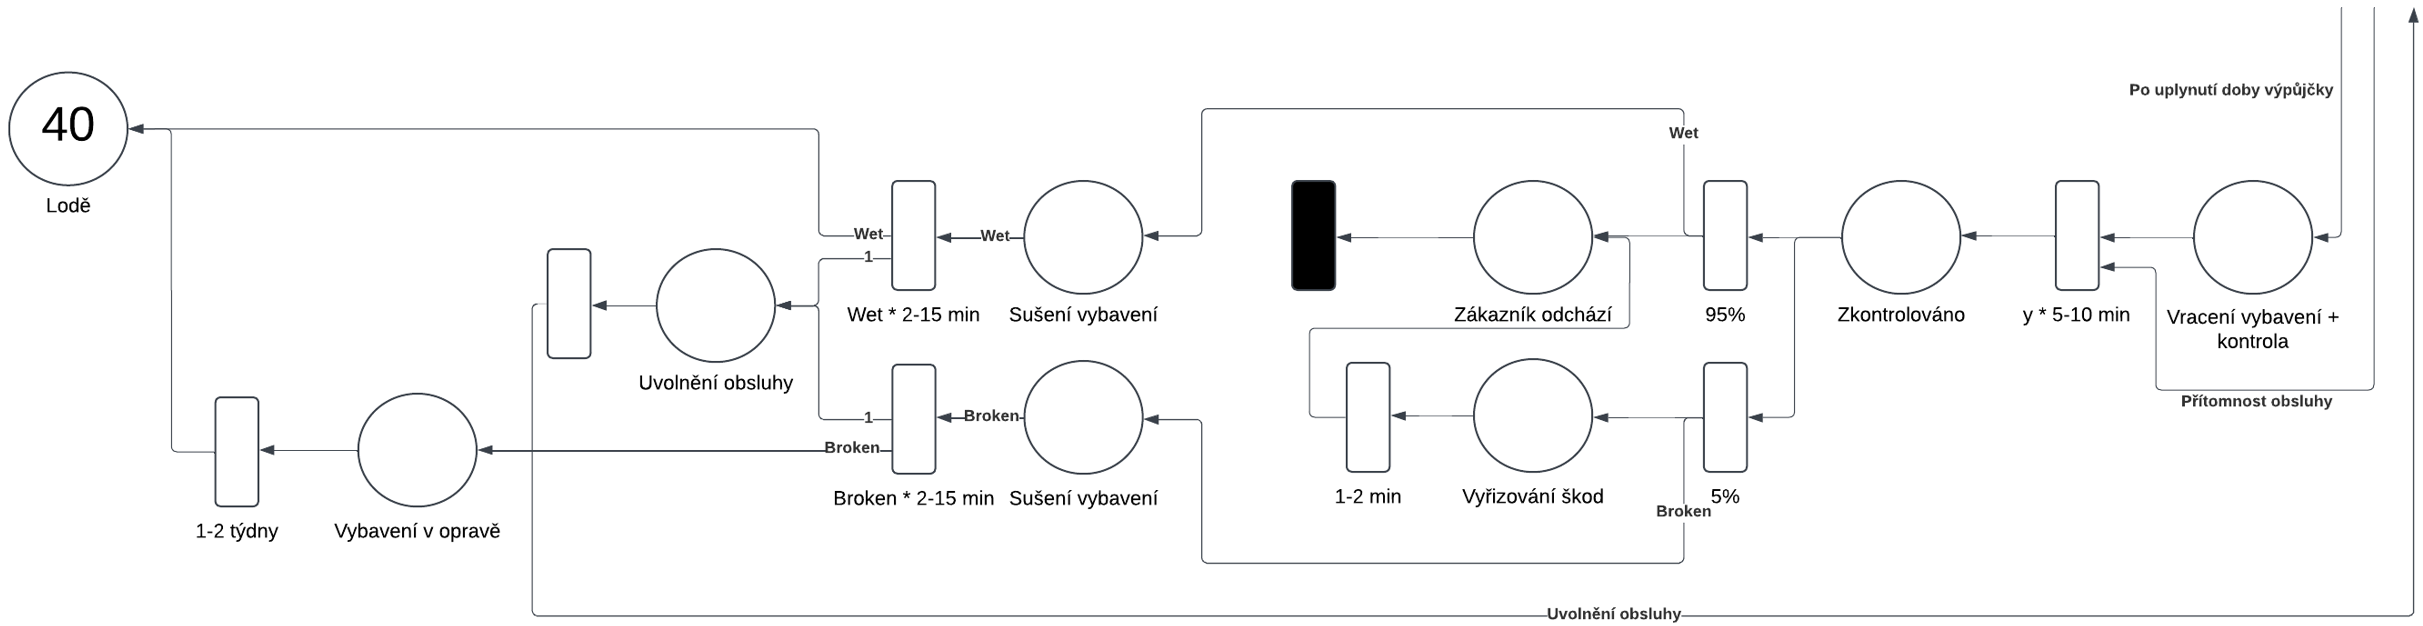
\includegraphics[width=1.0\linewidth]{images/vraceni.png}
    \caption{Vrácení zboží po vypůjčení}
    \label{fig:return}
\end{figure}


\newpage

\section{Koncepce implementace}
Program se skládá ze dvou generátorů rezervací (jednotlivci a větší skupinky) pro vypůjčení vybavení. Spouští se simulace jednoho roku, aneb 12 měsíců (jeden měsíc je považován jako 30 dní), kde podle nastavení generátoru jsou vytvářeny rezervace. Rezervace jsou kontrolovány s dostupností vybavení a domlouvání termínu výpůjčky. Dostupné vybavení je implementované pomocí skladu o kapacitě zvolené argumentem (v základu 40). Zákazníci jsou implementováni pomocí FIFO front, do kterých se řadí, pokud je obsluha dočasně zaneprázdněna zpracováváním jiných požadavků. Následně je implementována obsluha zákazníka, jak při předávání půjčeného vybavení, tak při následném přebírání, včetně případného zajištění opravy vybavení.

\subsection{Inicializace simulace}

\begin{algorithm}[H]
    \caption{Inicializace simulace}\label{alg:initialization}
    \SetAlgoLined
    \KwData{Argumenty z příkazové řádky}
        Zpracování argumentů z příkazové řádky\;
        Určení frekvence příchodu uživatelů\;
        Inicializace skladu lodí s počtem daným argumentem\;
        Nastavení doby trvání simulace\;
        Aktivace generátorů jednotlivců a velkých skupin\;
\end{algorithm}

\subsection{Popis implementace generátoru rezervací}

\begin{algorithm}[H]
    \caption{Chování Generátoru rezervací}\label{alg:reservation_generator}
    \KwOut{Aktivuje nové rezervace během aktivní sezóny}
    \BlankLine
    \If{\texttt{Čas < Délka sezóny}}{
        Vytvoření rezervace\;
        Naplánuj další aktivaci na \texttt{Čas v simulaci + ReservationTime()}\;
    }
\end{algorithm}

\subsection{Vytvoření rezervace}

\begin{algorithm}[H]
    \caption{Vytvoření rezervace}\label{alg:create_reservation}
    \KwIn{Počet lodí (\texttt{requestedBoat}), čas začátku (\texttt{start}), čas konce (\texttt{end})}
    \KwOut{Nová rezervace nebo odmítnutí kvůli nedostupnosti lodí}
    \BlankLine
    \If{\texttt{Je čas dostupný na který chce zákazník rezervovat}}{
        Vytvoř novou rezervaci\;
        Přidej rezervaci do seznamu rezervací\;
        Aktivuj rezervaci v čase kdy to začíná\;
    }
    \Else{
        Najdi nejbližší volný čas pro rezervaci\;
        \If{Pokud existuje dostatečný čas pro vypůjčení}{
            Vytvoř novou rezervaci s \texttt{earliestAvailable} jako časem začátku\;
            Přidej rezervaci do seznamu rezervací\;
            Aktivuj rezervaci v čase \texttt{earliestAvailable}\;
        }
        \Else{
            Rezervace je odmítnuta kvůli nedostupnosti lodí\;
        }
    }
\end{algorithm}

\subsection{Proces po rezervaci}

\begin{algorithm}[H]
    \caption{Proces po rezervaci a vrácení lodí}\label{alg:reservation}
    \SetAlgoLined
    Počkej na čas, který je rezervovaný\;
    Vstup do půjčovny lodí\;
    Počkej na vyřízení požadavku, poučení a demonstrování od zaměstnance\;
    Počkej na konec doby vypůjčení\;
    Vrať se do půjčovny\;
    Probíhá kontrola lodí\;
    Urči počet \(\text{rozbitých}\) lodí\;
    \If{(Pokud jsou nějaké lodě poškozené)}{
        Zákazník $\to$ Doplať poplatek za poškozené lodě\;
        Zaměstnanec $\to$ Počkej na konec vysušení lodí\;
        Pošli poškozené lodě do opravy
    }
    Počkej na konec vysušení lodí
\end{algorithm}

\subsection{Vysoušení lodí}

\begin{algorithm}[H]
    \caption{Proces vysoušení lodí}\label{alg:drying}
    \SetAlgoLined
    \textbf{Proces} \texttt{boatDrying(počet lodí k vysušení)}\;
    Počkej na konec vysoušení lodí\;
    Vrať lodě do skladu pro další vypůjčení\;
\end{algorithm}

\subsection{Oprava vybavení}

\begin{algorithm}[H]
    \caption{Proces opravy vybavení}\label{alg:repair}
    \SetAlgoLined
    \textbf{Proces} \texttt{boatRepair(počet poškozených lodí)}\;
    Počkej na konec opravu lodí\;
    Vrať lodě do skladu pro další vypůjčení\;
\end{algorithm}

\subsection{Volba počtu půjčeného vybavení}

\begin{algorithm}[H]
\caption{Algoritmus pro výběr počtu půjčených lodí}
\SetAlgoLined
\If{velká skupina}{
    množství chtěných lodí $\leftarrow$ Exp$(10) + 10$\;
    \Return $\min$(množství chtěných lodí, 40)\;
}
\Else{
    množství chtěných lodí $\leftarrow$ Exp$(2) + 1$\;
    \Return $\min$(množství chtěných lodí, 10)\;
}
\end{algorithm}

\subsection{Interval rezervace}

\begin{algorithm}[H]
\caption{Proces generování rezervací pomocí intervalů}
\SetAlgoLined
\If{Čas v simulaci $\leq$ První měsíc \textbf{nebo} Čas v simulaci $\geq$ Poslední měsíc}{
    \Return Exp$(2 \times x)$\;
}
\Else{
    \Return Exp$(x)$\;
}
\end{algorithm}

\newpage

\section{Architektura simulačního modelu}
Při návrhu simulačního modelu byl kladen důraz na realistické zobrazení procesů spojených s výpůjčkou lodí v půjčovně. Model byl navržen tak, aby zohledňoval nejen různé typy zákazníků a jejich chování, ale i sezónnost a omezenou kapacitu skladu lodí. Taktéž bylo bráno v úvahu možné poškození lodí, které může nastat v 5\% případů vypůjčení vybavení. Tento aspekt je zahrnut do procesu vracení vybavení a následného řešení oprav.

Model rovněž bere v úvahu sezónnost, která ovlivňuje počet rezervací. Na začátku a na konci sezóny je příliv zákazníků nižší, zatímco během vrcholu sezóny (zejména v letních měsících) je provoz půjčovny výrazně intenzivnější. Pro simulaci sezónnosti byl zvolen přístup s proměnlivou intenzitou generování rezervací, přičemž byl kladen důraz na realistické rozložení rezervací v čase.

Dalším významným aspektem modelu je omezená kapacita skladu lodí, která činí 40 kusů. Tento limit často vede k nutnosti zařazení zákazníků do fronty, pokud poptávka přesahuje dostupné zdroje. Pokud se však nevejde do časového intervalu, než by chtěl začít rezervaci, tak odchází.

\subsection{Mapování abstraktního modelu na simulační}
Vytváření zákazníků, respektive rezervací je řešeno pomocí tříd \textbf{ReservationGenerator} a \textbf{BigReservationGenerator}. Obě tyhle třídy používají svůj vlastní časový interval při generování daného typu zákazníka (ať už jednotlivce nebo větší skupinky). Následně volají funkci \textbf{CreateReservation}

CreateReservation vytváří rezervace s daným začátkem a koncem, který přidává do seznamu rezervací. Pokud již existuje rezervace v daném termínu, snaží se najít dřívější termín. Pokud není dostatečný časový prostor pro vytvoření rezervace, tak kvůli nedostupnosti lodí zákazník odchází.

Reservation řeší hlavní část programu, kde je započato čekání na daný termín vypůjčení, který je 7-30 dní od vzniku rezervace. Poté se odebere ze skladu potřebné množství lodí a začne samotná obslužní linka [1, snímek 144] obsluhy půjčovny.

Při vrácení zboží u každého kusu může nastat v 5\% případů poškození vybavení či jeho ztráta. V případě, že některé lodě jsou poškozené, prodavač se zákazníkem musí vyřešit právní náležitosti a doplatek za způsobené škody a potom se lodě vysuší a začne nová instance \textbf{boatRepair}. Tato instance čeká na opravu daných lodí a pak je vrací zpět do skladu.

Je zřetelné, že ne všechny lodě budou poškozené a tak se pro ty které poškozené nebyly vytváří instanci třídy \textbf{boatDrying}, která po uplynutí daného času sušení lodě, což dělá v našem případě hodnotu danou počtem lodí vynásobeným 2 až 15 minutami, přesune vybavení zpátky do skladu.

\newpage 

\section{Experimentování}
Cílem experimentování je analyzovat chování systému provozu půjčovny vodáckého vybavení a najít klíčové faktory, které ovlivňují její efektivitu a kvalitu služeb. Pomocí navrženého simulačního modelu lze efektivně testovat a zkoumat různé situace a jejich dopady na chod půjčovny. Zároveň lze identifikovat případné problémy, které se vyskytují v dosavadním modelu půjčovny, případně navrhnout jak lze tyto problémy optimalizovat. 

Před začátkem experimentování je však nezbytné uvést počáteční úvahy, v jakých sekcích půjčovny se mohou vyskytovat mezery, a co by na nich mohlo jít vylepšit. Například bylo by možné nalézt optimální množství dostupného vybavení půjčovny? Zvládne půjčovna náhlý nápor zákazníku vzhledem k probíhající reklamní kampani? Jak ovlivňuje délka a kvalita sezóny chod půjčovny a jak bude ovlivněná změnou délky vypůjčení vybavení?

Na zodpovězení těchto a dalších otázek se zaměříme v následujícím textu.

\subsection{Dokumentace jednotlivých experimentů}
\subsubsection{Experiment 1 - vliv dostupného vybavení na provoz půjčovny}
Cílem prvního experimentu je nalezení optimálního množství dostupného vybavení půjčovny, aby došlo ke snížení čekací doby, což má přímý vliv na zvýšení spokojenosti zákazníků. V základu tahle hodnota odpovídá číslu 40. Při průměrném počtu dvou zákazníků za den, se však tvoří fronty na rezervaci vybavení. Simulace byla spouštěna se vstupními parametry níže v tabulce \ref{tab:simulation_stats1}. Pokud pro potřeby experimentu zvolíme neomezenou dostupnost vybavení půjčovny, pak zjistíme, že současně bylo využito maximálně 50 kusů vybavení, tedy ideální dostupnost lodí bude 50. 

% Možná by se vyplatilo popsat ty hodnoty jak se měnili, ...
\begin{table}[h!]
    \centering
    \caption{Vstupní hodnoty a statistiky experimentu 1}
    \label{tab:simulation_stats1}
    \begin{tabular}{|c|c|c|c|c|}
        \hline
        \textbf{Zákazníci / den} & \textbf{Lodě (ks)} & \textbf{Prům. čas ve frontě (min)} & \textbf{Max. délka fronty} & \textbf{Odmítnuté}\\ \hline
        2 & 30 & 494.3 & 3 & 49 \\ \hline
        2 & 35 & 1077.2 & 2 & 17 \\ \hline
        2 & 40 & 324.4 & 1 & 7 \\ \hline
        2 & 45 & 38.1 & 2 & 8 \\ \hline
        2 & 50 & 0 & 0 & 9 \\ \hline
    \end{tabular}
\end{table}

\subsubsection{Experiment 2 - vliv reklamní kampaně na provoz půjčovny}
Cílem tohoto experimentu bylo zkoumat chování systému, po spuštění reklamní kampaně, jejíž příčinou by bylo nárazové zvýšení průměrného počtu zákazníků po dobu jedné sezóny. Z experimentů je zřetelné, že již pro 4 zákazníky za den výrazně vzroste průměrná doba, kterou zákazník musí čekat ve frontě na dostupné vybavení. Co bylo však nečekané je, že při zvýšení počtu zákazníků se průměrný čas ve frontě může také snížit. 
Pro 3 a 4 zákazníky za den se doba čekání ve frontě postupně zvyšovala, ale od 5 a více zákazníků se průměrná doba čekání ve frontě opět snížila a držela se kolem relativně stabilních hodnot. To je dáno především tím, že pokud zákazníkům nevyhovuje volný termín, tak odchází. Při vyšším počtu zákazníků bude větší počet neobsloužených, ale zákazníci se lépe řadí do volných termínů.
Sledovali jsme také vytížení zaměstnance, ale zjistili jsme, že s aktuálním počtem dostupných lodí je vytížení zaměstnance akceptovatelné i při zvýšení poptávky, problém je v takovém případě pouze s počtem dostupných lodí.
\begin{table}[h!]
    \centering
    \caption{Vstupní hodnoty a statistiky experimentu 2}
    \label{tab:simulation_stats2}
    \begin{tabular}{|c|c|c|c|c|}
        \hline
        \textbf{Zákazníci / den} & \textbf{Počet lodí} & \textbf{Prům. čas ve frontě (hod)} & \textbf{Max. délka fronty} & \textbf{Odmítnuté}\\ \hline
        2 & 40 & 5.4 & 1 & 7\\ \hline
        4 & 40 & 17.35 & 5 & 236\\ \hline
        10 & 40 & 16.3 & 5 & 1078\\ \hline
    \end{tabular}
\end{table}

\subsubsection{Experiment 3 - vliv délky sezóny na provoz půjčovny}
Cílem tohoto experimentu bylo zkoumat, jaký vliv má změna délky sezóny na provoz půjčovny lodí. Konkrétně jsme se zaměřili na změnu délky sezóny z původních 6 a půl měsíce na zkrácených 3 a půl měsíce a také prodloužených 8 měsíců, abychom zjistili, jak tato změna ovlivní vytíženost vybavení, množství příchozích zákazníků, délku fronty a celkovou efektivitu systému.

Z experimentu je patrné, že prodloužení délky sezóny má přímý vliv na průměrné využití vybavení a také s přibývajícím počtem zákazníků také na délku fronty. Při délce sezóny 6 a půl měsíce bylo průměrné využití lodí rovných 12 kusů. Nejdelší sezóna s 8 měsíci přinesla nejvyšší hodnoty s průměrným využitím lodí až 15.3 kusů po celý rok. Jak by se dalo očekávat, s nejkratší dobou trvání aktivní sezóny bylo průměrné využití lodí v půjčovně nejnižší.

\begin{table}[h!]
    \centering
    \caption{Vstupní hodnoty a statistiky experimentu 3}
    \label{tab:simulation_stats3}
    \begin{tabular}{|c|c|c|c|}
        \hline
        \textbf{Zákazníci / sezóna} & \textbf{Prům. využití lodí} & \textbf{Fronta (zákazníci)} & \textbf{Délka sezóny (měsíce)} \\ \hline
        319 & 12 & 2 & 6.5 \\ \hline
        142 & 5.2 & 2 & 3.5\\ \hline
        412 & 15.3 & 3 & 8\\ \hline
    \end{tabular}
\end{table}

\subsubsection{Experiment 4 - vliv zvýšení poptávky velkých skupin na chování systému}
Cílem tohoto experimentu bylo zkoumat, jaký vliv na chování systému má zvýšení poptávky ze strany velkých skupin (zájezdů, škol apod.). Analyzovali jsme, jaký vliv má různý čas generování skupin (s exponenciálním rozdělením s různými vstupními parametry), jak ovlivňují průměrnou dobu strávenou ve frontě a její maximální délku. Tento experiment slouží k porozumění, co by se stalo, když by se zvýšila poptávka velkých skupin, například školní zájezdy před letními prázdninami a jaký by to mělo vliv na dostupnost vybavení, nutnosti odmítnout nějaké zákazníky s ohledem na nedostupnost vybavení a podobně.

S vyšším množstvím zájezdů nebo skupinových vypůjčení se zvyšuje úměrně průměrný čas strávený ve frontě na lodě spolu s odmítnutými rezervacemi z důvodu přeplnění termínů a nedostatečnými zdroji půjčovny.
\begin{table}[h!]
    \centering
    \caption{Vstupní hodnoty a statistiky experimentu 4}
    \label{tab:simulation_stats2}
    \begin{tabular}{|c|c|c|c|c|}
        \hline
        \textbf{Časy generování skupin} & \textbf{Počet lodí} & \textbf{Prům. čas ve frontě (hod)} & \textbf{Max. délka fronty} & \textbf{Odmítnuté} \\ \hline
        Exp(20 * x) & 40 & 5.4 & 1 & 7 \\ \hline
        Exp(5 * x) & 40 & 8.6 & 3 & 20\\ \hline
        Exp(x) & 40 & 15.3 & 2 & 82 \\ \hline
    \end{tabular}
\end{table}

\subsection{Závěry experimentů}
Byly provedeny celkem 4 experimenty zaměřené na různé aspekty ovlivňující provoz a funkci půjčovny lodí, včetně vlivu počtu dostupného vybavení, frekvence vzniku nových rezervací, jak jednotlivců, tak také i skupin a délky sezóny. 

Z těchto experimentů jsme odvodili, že při zvýšení počtu lodí ze 40 na 50 došlo ke snížení průměrné doby čekání zákazníků a zároveň také počtu odmítnutých zákazníků s ohledem na nedostupnost dalšího vybavení. Pro optimalizaci systému je tedy maximální počet dostupného vybavení zcela zásadní.

Zároveň jsme také došli k závěru, že při spuštění reklamní kampaně a následnému zvýšení frekvence příchodu nových zákazníků dochází k zatížení systému a s tím společné zvýšení doby čekání zákazníku ve frontě a obrovské množství odmítnutých zákazníků. Podle těchto experimentů by se tedy dalo určit, jaká reklamní kampaň (respektive příbytek nových zákazníků) by byla dostatečná, případně, jaká by nevynášela očekávané výsledky, protože by docházelo jen k dalšímu odmítání zákazníků. S reklamní kampaní nám sice poměrně vzroste počet obsloužených zákazníků, ale počet odmítnutých zákazníku strmě stoupá.

Podobně je tomu tak i se zvýšením frekvence příchodu velkých skupin, kde opět zvýšení poměrně výrazně ovlivňuje průměrný čas strávený ve frontě a nutnost odmítnout některé zákazníky s ohledem na nedostupnost vybavení. 

S prodloužením délky sezóny došlo k nárustu průměrného využití lodí za rok a spolu s tím došlo i k mírnému nárustu průměrné délky fronty.

Z experimentů lze tedy odvodit, že pro optimální chování systému je nutné udržovat rovnováhu mezi počtem dostupného vybavení v půjčovně, intenzitou rezervací jak jednotlivců, tak velkých skupin.

\subsection{Spouštění jednotlivých experimentů}
\subsubsection{Experiment 1}
\begin{verbatim}
    make experiment1
\end{verbatim}
\subsubsection{Experiment 2}
\begin{verbatim}
    make experiment2
\end{verbatim}
\subsubsection{Experiment 3}
\begin{verbatim}
    make experiment3
\end{verbatim}
\subsubsection{Experiment 4}
Pro spuštění experimentu 4 je potřeba upravit hodnoty nastavené v kódu u návratové hodnoty funkce \texttt{BigReservationInterval()} na požadovanou hodnotu.
\newpage
\section{Závěr}
Cílem této práce bylo navrhnout, implementovat a analyzovat simulační model půjčovny vodáckého vybavení. Tento model měl za úkol co nejrealističtěji zobrazit chování systému s ohledem na sezónnost, omezenou kapacitu vybavení a různé typy zákazníků. Na základě provedených experimentů lze vyvodit několik důležitých závěrů.

Délka sezóny od poloviny dubna do konce října byla shledána jako dostatečná pro efektivní provoz půjčovny. Při prodloužení sezóny na více než osm měsíců se však zvyšuje vytížení systému, což může vést k přetížení zdrojů a prodloužení doby čekání.

Z pohledu provozu půjčovny se potvrdilo, že průměrná míra poškození lodí, která činí 5\% z vypůjčeného vybavení, má vliv na dostupnost lodí a potřebu jejich oprav. Přestože současný systém opravy vybavení zajišťuje jejich rychlé navrácení do provozu, při zvýšené poptávce může dojít k přetížení opravného procesu.

Závěrem lze říci, že navržený model poskytuje realistický obraz o fungování půjčovny vodáckého vybavení a umožňuje efektivně testovat různé scénáře provozu. Výsledky experimentů mohou sloužit jako podklad pro rozhodování o optimalizaci dostupného vybavení, plánování sezónního provozu a zajištění kvalitních služeb zákazníkům.

\newpage

\rhead{Bibliografie}

\renewcommand{\refname}{Bibliografie}
\begin{thebibliography}{9}

    \bibitem{Peringer2024} Peringer P., Hrubý M.: 
    Modelování a simulace – prezentace do předmětu Modelování a Simulace na Fakultě informačních technologií VUT v Brně. [online], 2024, [viděno 28.11.2024]. Dostupné z: \url{https://www.fit.vut.cz/person/peringer/public/IMS/prednasky/IMS.pdf}

    \bibitem{simlib}
    Peringer P.: \textit{SIMLIB – Simulační knihovna pro modelování a simulaci systémů hromadné obsluhy.} Vývoj od roku 1991, s příspěvky D. Lesky (1995–1997, numerické metody) a D. Martinka (2000–2001, fuzzy rozšíření). [online], 2023, [viděno 28.11.2024]. Dostupné z: \url{https://www.fit.vut.cz/person/peringer/public/SIMLIB/}

    \bibitem{GitHub2024} GitHub:
    GitHub Dashboard – online platforma pro verzování a správu projektů. [online], 2024, [viděno 29.11.2024]. Dostupné z: \url{https://github.com/dashboard}

    \bibitem{Peringer2022} Peringer P.:
    Modelování a simulace IMS – Studijní opora. [online], 2. února 2022, [viděno 29.11.2024]. Dostupné z: \url{https://www.fit.vut.cz/person/peringer/public/IMS/prednasky/IMS.pdf}


\end{thebibliography}

\end{document}
